The main purpose of this project is to predict the risk, at the application time of the loan, that a person will default the terms of this precise loan (he is asking for) according to the his personal data (location, gender, employment, etc.), to his past experience of loan (if he has) and finally according to the similar past loans that other people asked for.

\section{Estimation of the risk}
	To estimate this risk, several informations are going to be used :
	\begin{itemize}[label=$\bullet$]
	    \item In case it is the first time the person plans to borrow money, then he must subscript to Bitbond platform and give several informations about him-self before applying for a loan. In that case we do not know anything about him except those precise informations. Therefore we can only focus on those informations (and take them for granted) and compare them with other people informations.
	    \item In case it is not the first time the person is asking for a loan, then we have his personal informations and also informations about his past experiences of borrowing. Thus we can focus on his loan history and also look to other people who asked for the same kind of loan.
	\end{itemize}

\paragraph{Model mapping spaces :}
	To predict the risk of default, we built a model (see section \ref{sec:models}) mapping the space of loans to the space of labels : $$f_\theta:\mathcal{X}\rightarrow \mathcal{Y}$$
	$$f_\theta(X)\mapsto Y$$
	With :
	\begin{itemize}[label=$\bullet$]
		\item $X\in\mathcal{X}$ the matrix of loans of shape $(n,p)$ ($n$ loans described by $p$ features) :
		$$
		\begin{array}{cc}
			\begin{array}{ccc}
				 & ~~~~feature_1 & feature_p\\
				 & ~~~~\downarrow & \downarrow
			\end{array}\\
				X =
			\left(
				\begin{array}{ccc}
					x_{1,1} & \dots & x_{1,p}\\
					\vdots &  & \vdots\\
					x_{n,1} & \dots & x_{n,p}
				\end{array}
			\right) & \begin{array}{c}
		  \leftarrow loan_1\\
		  \\
		  \leftarrow loan_n
		  \end{array}
		  \end{array}$$
		\item $Y\in\mathcal{Y}$ the vector of labels of shape $(n,1)$ : $$\mathcal{Y} = \{0, 1\}$$
	\end{itemize}

	\begin{figure}[h]
		\centering
		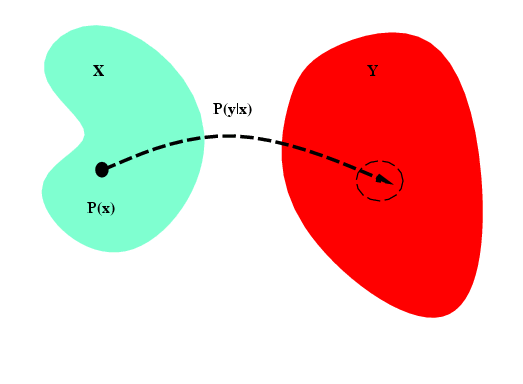
\includegraphics[width=0.7\textwidth]{images/mapping_proba.png}
		\caption{Mapping between the set $\mathcal{X}$ and $\mathcal{Y}$.}
		\label{fig:mapping_proba}
	\end{figure}

	We are trying to estimate the probability $p(Y|X)$ assuming that $X$ and $Y$ share a joint distribution (like described in figure \ref{fig:mapping_proba}).

\newpage

\paragraph{Minimization of the risk :}
	The model which is minimizing the regularized empirical risk, can be found by solving the following optimization problem :
	$$\theta^*=argmin_\theta\sum_{i=1}^n l(y_i,f_\theta(x_i)) + \lambda\Omega(\theta)$$
	Where :
	\begin{itemize}
		\item $l(y_i,f_\theta(x_i))$ is the loss function between the true label $y_i$ and the predicted one $f_\theta(x_i)$
		\item $\lambda\Omega(\theta)$ is the regularization parameter to prevent from over-fitting.
	\end{itemize}

\section{Evaluation}
	The model built will be evaluated by computing the \textbf{log-loss} on predicted probabilities during a \textbf{5-fold cross validation}.

	\subsection{Logistic loss}
		The log-loss measures the accuracy of a classifier. We use it when the model outputs a probability for each class, rather than just the most likely class. That is basically what we aim to do by predicting a probability of defaulting that estimates this precise risk.\\

		The log-loss is a measurement of accuracy that incorporates the idea of probabilistic confidence. It is intimately tied to information theory : log-loss is the cross entropy between the distribution of the true labels and the predictions. Intuitively speaking, entropy measures the unpredictability of something. Cross entropy incorporate the entropy of the true distribution, plus the extra unpredictability when we assume a different distribution than the true distribution. So log-loss is an information-theoretic measure to gauge the ``extra noise'' that comes from using a predictor as opposed to the true labels. The use of log on the error provides extreme punishments for being both confident and wrong. In the worst possible case, a single prediction that something is definitely true when it is actually false will add infinite to your error score and make every other entry pointless. By minimizing the cross entropy, we maximizes the accuracy of the classifier. The mathematical definition of the log-loss is visible below :
		$$L = -\frac{1}{n}\sum_{i=1}^{n}[y_i\log(p_i)+(1-y_i)\log(1-p_i)]$$

	\subsection{5-fold cross validation}
		The model built will be evaluated with a 5-fold cross validation. The entire dataset is split into 5 subsamples and each subsample is used once to validate the model and four times to train it. In figure \ref{fig:5_fold_cv} you can see how each subsample of the whole dataset is used in each fold.

	\begin{figure}[h]
		\centering
		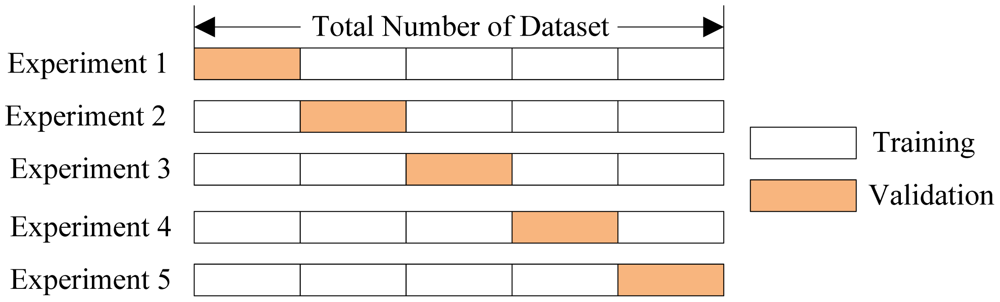
\includegraphics[width=\textwidth]{images/5_fold_cv.png}
		\caption{Each subsample is used once for validation and four times for training.}
		\label{fig:5_fold_cv}
	\end{figure}

	In each fold, one borrower must be either in the training set or the testing set but never in both, to prevent from over fitting (see section \ref{sec:data} for further informations on the data). Here is what is done in each fold (also visible in figure \ref{fig:cv_process}):
	\begin{enumerate}
		\item Build a classifier on a training set
		\item Predict the probabilities of each label on a validation set
		\item Compute the logistic loss
		\item Compute the area under the Receiver Operating Characteristic curve (ROC-AUC score)
	\end{enumerate}

	\begin{figure}[h]
		\centering
		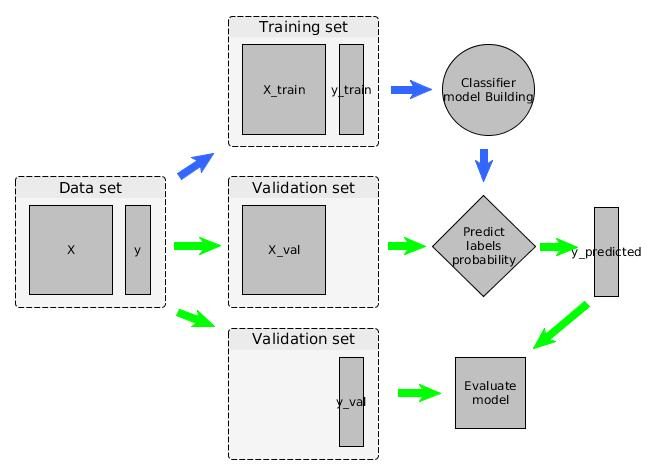
\includegraphics[width=\textwidth]{images/cv_process.jpg}
		\caption{What is done during one fold of cross validation.}
		\label{fig:cv_process}
	\end{figure}

	\subsection{Area Under the Receiver Operating Characteristic Curve (AUC-ROC)}
		To evaluate the model built, we also compute the area under the Receiver Operating Characteristic curve.
		À développer!

\section{Data}\label{sec:data}
	The dataset we are using is provided by the Bitbond lending platform. For confidentiality reasons, the data are anonymized. The dataset contains 2177 loans described by : a loan status, a loan term in months, a loan purpose from a given set, a free text project description, a loan amount, a currency (Bitcoin or USD), the number of rates to pay and those already paid, the publishing and funding time of the loan, a borrower ID, the borrower's employment, the borrower's net income in local currency, the borrower's address (latitude and longitude), some information about the social media connection between the borrower and the Bitbond page (only boolean, due to anonymization).\\

	Among those 2177 loans :
	\begin{itemize}
		\item 608 loans have either the status defaulted (49), fully paid back (391), charged off (119) or 90 days late (49)
		\item We consider only those 608 loans to build our classification model (with a proportion of fully paid back label of 65\% against the rest)
		\item There are 521 distinct borrowers whose 446 have an address defined by their latitude and longitude
	\end{itemize}